\documentclass[11pt,usenames,dvipsnames,
hyperref={pdfencoding=auto,psdextra}]{beamer}
\def\showTODOs{}


\usepackage{gensymb}

\newcommand*{\listsofb}[1]{\mathcal{L} (#1)}
\newcommand*{\listsof}{\mathcal{L}~}

\newcommand{\None}{\emptyset}
\newcommand{\Some}[1]{\degree\kern-0.5ex#1}
\newcommand{\lnil}{\ensuremath{[]}}

\newcommand*{\match}{\textbf{match}~}
\newcommand*{\withl}{\textbf{[}~}
\newcommand*{\withr}{~\textbf{]}}
\newcommand*{\withm}{\quad\textbf{|}\quad}
\newcommand*{\llet}{\textbf{let}~}
\newcommand*{\lin}{\textbf{in}~}
\newcommand{\ITE}[3]{\textbf{if}~{#1}~\textbf{then}~{#2}~\textbf{else}~{#3}}

\newcommand{\Type}{\mathbb{T}}
\newcommand{\Prop}{\mathbb{P}}
\newcommand{\bool}{\mathbb{B}}
\newcommand{\btrue}{\mathsf{T}}
\newcommand{\bfalse}{\mathsf{F}}
\newcommand{\andb}{\&\&}
\newcommand{\orb}{||}
\newcommand{\notb}{!}
\newcommand{\nat}{\mathbb{N}}
\newcommand{\natS}{1 + }
\newcommand{\length}[1]{|#1|}

\newcommand{\con}{\mathop{{+}\!\!\!{+}}}
\newcommand{\rev}{\mathsf{rev}}
\newcommand{\opt}[1]{\mathcal{O}{#1}}

\newcommand{\eqb}[2]{#1\overset{?}{=}#2}

\usepackage[english]{babel}
\usepackage{lipsum}
\usepackage{mathtools}
\usepackage{pifont}
\usepackage{wasysym}
\usepackage{booktabs}
\usepackage{multirow}
\usepackage[absolute,overlay]{textpos}
\usepackage{proof}
\usepackage{amsmath}
%\usepackage[utf8]{inputenc}
\usepackage{listings}
\usepackage{tikz}
\usetikzlibrary{automata,trees,calc,arrows.meta,positioning,decorations.pathreplacing,bending,shapes.geometric, intersections, hobby}
\usetheme{Berlin}
\usepackage{cite}
\usepackage{cancel}
\usepackage{xsavebox}
\usepackage[normalem]{ulem}
\usepackage{array}
%\usepackage{wasysym}
\usepackage{stmaryrd}
\usepackage{pgfplots}
\usepackage{ifthen}
\usepackage{latexsym}
\usepackage{turnstile}


\pgfplotsset{compat=1.16}

%some nicer colour scheme
\definecolor{craneorange}{RGB}{237, 142, 26}
\definecolor{craneblue}{RGB}{0,0,0}

\setbeamercolor{structure}{fg=craneblue}

\setbeamercolor{palette primary}{fg=craneblue,bg=craneorange!70}
\setbeamercolor{palette secondary}{fg=craneblue,bg=craneorange!80}
\setbeamercolor{palette tertiary}{fg=craneblue,bg=craneorange!90}
\setbeamercolor{palette quaternary}{fg=craneblue,bg=craneorange}

\setbeamercolor{titlelike}{parent=palette quaternary}

\setbeamercolor{block title}{fg=craneblue,bg=craneorange}
\setbeamercolor{block title alerted}{use=alerted text,fg=craneblue,bg=alerted text.fg!75!bg}
\setbeamercolor{block title example}{use=example text,fg=craneblue,bg=example text.fg!75!bg}

\setbeamercolor{block body}{parent=normal text,use=block title,bg=block title.bg!15!bg}
\setbeamercolor{block body alerted}{parent=normal text,use=block title alerted,bg=block title alerted.bg!15!bg}
\setbeamercolor{block body example}{parent=normal text,use=block title example,bg=block title example.bg!15!bg}

\setbeamercolor{sidebar}{bg=craneorange!70}

\setbeamercolor{palette sidebar primary}{fg=craneblue}
\setbeamercolor{palette sidebar secondary}{fg=craneblue!75}
\setbeamercolor{palette sidebar tertiary}{fg=craneblue!75}
\setbeamercolor{palette sidebar quaternary}{fg=craneblue}

\setbeamercolor*{separation line}{}
\setbeamercolor*{fine separation line}{}

\setbeamercolor{frametitle}{bg=white}

%no frame numbering when using framebreaks
\setbeamertemplate{frametitle continuation}{}

%no total frame number
\setbeamertemplate{footline}{% 
  \hfill% 
  \usebeamercolor[fg]{page number in head/foot}% 
  \usebeamerfont{page number in head/foot}% 
  \insertframenumber%
  %\,/\,\inserttotalframenumber
  \kern1em\vskip2pt% 
}

%no subsection line
\setbeamertemplate{headline}
{%
  \begin{beamercolorbox}[colsep=1.5pt]{upper separation line head}
  \end{beamercolorbox}
  \begin{beamercolorbox}{section in head/foot}
    \vskip0pt\insertnavigation{\paperwidth}\vskip3pt
  \end{beamercolorbox}%
  \begin{beamercolorbox}[colsep=1.5pt]{lower separation line head}
  \end{beamercolorbox}
}

%highlight colours to be used throughout the presentation
\newcommand{\highlight}[1]{\color{blue}#1\color{black}}
\newcommand{\colorHOne}{\color{red}}
\newcommand{\colorHThree}{\color{violet}}
\newcommand{\colorHTwo}{\color{blue}}
\newcommand{\colorHFour}{\color{green}}

\newcommand{\colorTikzA}{red}
\newcommand{\colorTikzB}{cyan}
\newcommand{\colorTikzC}{blue}
\newcommand{\colorTikzD}{green}
\newcommand{\colorTikzE}{violet}

%don't count the title page
\let\otp\titlepage
\renewcommand{\titlepage}{\otp\addtocounter{framenumber}{-1}}

%a hide on=... option for tikz elements, where the usual ranges allowed by \only are allowed for ...
\tikzset{hide on/.code={\only<#1>{\pgfkeysalso{white}}}}

%don't want those nasty navigation symbols
\beamertemplatenavigationsymbolsempty


\newenvironment{tightcenter}{%
  \setlength\topsep{0pt}
  \setlength\parskip{0pt}
  \begin{center}
    }{%
  \end{center}
}

%table column types for fixed width
\newcolumntype{L}[1]{>{\raggedright\let\newline\\\arraybackslash\hspace{0pt}}m{#1}}
\newcolumntype{C}[1]{>{\centering\let\newline\\\arraybackslash\hspace{0pt}}m{#1}}
\newcolumntype{R}[1]{>{\raggedleft\let\newline\\\arraybackslash\hspace{0pt}}m{#1}}

\newcommand{\TODO}[1]{\ifthenelse{\isundefined{\showTODOs}}{}{\colorbox{red}{\LARGE TODO}:#1}}


%math stuff
\newcommand*{\Eq}{\text{Eq}}
\newcommand*{\N}{\mathbb{N}}
\newcommand*{\R}{\mathbb{R}}
\newcommand*{\Reach}{\text{Reach}}
\newcommand*{\norm}[1]{\left\lVert#1\right\rVert}
\newcommand*{\diff}{\text{d}}
\newcount\colveccount
\newcommand*\colvec[1]{
  \global\colveccount#1
  \begin{pmatrix}
    \colvecnext
  }
  \def\colvecnext#1{
    #1
    \global\advance\colveccount-1
    \ifnum\colveccount>0
      \\
      \expandafter\colvecnext
    \else
    \end{pmatrix}
  \fi
}


%prevent backup slides from appearing in the header
\makeatletter
\let\beamer@writeslidentry@miniframeson=\beamer@writeslidentry%
\def\beamer@writeslidentry@miniframesoff{%
  \expandafter\beamer@ifempty\expandafter{\beamer@framestartpage}{}% does not happen normally
  {%else
    % removed \addtocontents commands
    \clearpage\beamer@notesactions%
  }
}
\newcommand*{\miniframeson}{\let\beamer@writeslidentry=\beamer@writeslidentry@miniframeson}
\newcommand*{\miniframesoff}{\let\beamer@writeslidentry=\beamer@writeslidentry@miniframesoff}
\makeatother


%footnote without marker, for images
\newcommand\blfootnote[1]{%
  \begingroup
  \renewcommand\thefootnote{}\footnote{#1}%
  \addtocounter{footnote}{-1}%
  \endgroup
}

\newcommand{\bnfmid}{~\mid~}

\newcommand*{\PR}{\textbf{PR}}
\newcommand*{\sat}{\textbf{SAT}}
\newcommand*{\gennp}{\textbf{TMGenNP}}
\newcommand{\fsat}{\textbf{FSAT}}
\newcommand{\NP}{\textsf{NP}}

\newcommand{\defeq}{\coloneqq}

\newcommand{\redP}{\ensuremath{\preceq_p}}
\newcommand{\Clique}{\normalfont\textbf{Clique}}

\newcolumntype{C}{>{$}c<{$}}
\newcommand{\rewwin}[2]{
  \begin{tabular}{C|C|C}
    #1 \\ 
    \midrule #2
  \end{tabular}
}

\newcommand{\trewwin}[6]{
  \begin{tikzpicture}
    \draw[thick] (0, 0) -- (2.25, 0);
    \draw (0.75, -0.75) -- (0.75, 0.75);
    \draw (1.5, -0.75) -- (1.5, 0.75);
    \node at (0.375, 0.375) {\ensuremath{#1}};
    \node at (0.375, -0.375) {\ensuremath{#4}};
    \node at (1.125, 0.375) {\ensuremath{#2}};
    \node at (1.125, -0.375) {\ensuremath{#5}};
    \node at (1.875, 0.375) {\ensuremath{#3}};
    \node at (1.875, -0.375) {\ensuremath{#6}};
  \end{tikzpicture}
}

%workaround so that polarities on blanks have the same height as on other symbols
\newcommand*{\TallestContent}{\ensuremath{b \sigma_1}}% <-- This should be the tallest content

\newcommand{\polneg}[1]{\overleftarrow{#1\vphantom{\TallestContent}}}
\newcommand{\polpos}[1]{\overrightarrow{#1\vphantom{\TallestContent}}}
\newcommand{\polneut}[1]{\overline{#1\vphantom{\TallestContent}}}

\newcommand{\reprt}[1]{\ensuremath{\sim_t^{#1}}}
\newcommand{\reprtt}[2]{\ensuremath{\sim_t^{(#1, #2)}}}
\newcommand{\reprc}{\ensuremath{\sim_c}}



\newcommand{\strent}{\rightsquigarrow}
\newcommand{\constrent}{\overset{!}{\rightsquigarrow}}
\newcommand{\Rfinal}{R_{\text{final}}}

\newcommand{\blank}{\textbf{\textvisiblespace}}


\title{Towards a Formal Proof of the Cook-Levin Theorem}

\institute{Saarland University}
\date{15 April 2020\\[1ex]Final Bachelor Talk}
\author{Lennard Gäher\\[1mm] {\small{Advisor: Fabian Kunze}\\ \small{Supervisor: Prof.\ Smolka}}}

\begin{document}
\begin{frame}[plain]
  \titlepage
\end{frame}

\section{Introduction}
\begin{frame}{The Cook-Levin Theorem}
   
  \begin{center}
    \sat{} is \NP{}-complete\cite{Cook:1971:CTP:800157.805047, levin_theorem}.
  \end{center}
  \vspace{2ex}

  \begin{block}{\sat{}}
    Given a Boolean formula in conjunctive normal form, does there exist a satisfying assignment?
  \end{block}

  \vspace{2ex}
  \cite{Karp1972}: 21 more combinatorial \NP{}-complete problems

  \vspace{3ex}
  \onslide<2->{
    Mechanisation~\cite{gamboa:cook}: verified construction without connection to computational model (ACL2)
  }

\end{frame}

%\begin{frame}{Timeline}
  %\begin{tikzpicture}[overlay,remember picture]
    %\node[minimum width=\paperwidth,minimum height =\paperheight,anchor=north west] (a) {};
    %\draw[thick,->] ($(current page.north east)!0.5!(current page.north west) + (0, -0.57)$) -- ($(current page.south west)!0.5!(current page.south east) + (0, 1)$);
  %\end{tikzpicture}
  %\only<4->{\frametitle{Timeline: Mechanisation}}

  %\setlength{\TPHorizModule}{\textwidth}
  %\setlength{\TPVertModule}{\textwidth}
  %\begin{textblock}{0.5} (0.62, 0.15)
    %\small
    %\textbf{1965:} time/space complexity, hierarchy theorems, \ldots

    %\emph{On the Computational Complexity of Algorithms}

    %Hartmanis and Stearns\\
    %\onslide<4->{
      %$~$\\
      %{
        %\colorHTwo{}
        %mechanisation without reference to concrete model (Matita)~\cite{asperti:reverse_complexity}
      %}
    %}
  %\end{textblock}

    %\begin{textblock}{0.5} (0.05, 0.45)
      %\onslide<2->{
        %\small 
        %\textbf{1971:} Cook-Levin Theorem

        %\emph{The Complexity of Theorem-Proving Procedures}

        %Stephen A.\ Cook\\
        %\onslide<5->{
          %$~$\\
          %{ 
            %\colorHTwo{}
            %
          %}
        %}
      %}
    %\end{textblock}

    %\begin{textblock}{0.5} (0.62, 0.6)
    %\onslide<3->{
        %\small
        %\textbf{1972:} Karp's 21 NP-complete problems

        %\emph{Reducibility Among Combinatorial Problems}

        %Richard M.\ Karp
      %}
    %\end{textblock}
%\end{frame}

\begin{frame}{Our Computational Model}
  Prevalent computational model: Turing machines 
  $~$\\[5ex]
  \begin{quote}
    Turing machines as model of computation are inherently infeasible for the formalisation of any computability- or complexity-theoretic result
  \end{quote}
  \raggedleft{} \cite{ForsterEtAl:2019:VerifiedTMs}

  \raggedright{}
  Here: use $\lambda$-calculus L

  Supported by: 
  \begin{itemize}
    \item reasonability of L~\cite{ForsterKunzeRoth:2019:wcbv-Reasonable}
    \item extraction mechanism in Coq~\cite{ForsterKunze:2019:Certifying-extraction}
  \end{itemize}

  size explosion: \textbf{``time bounds space'' does not hold}
\end{frame}

\newcommand{\Term}{\textsf{term}}
%\begin{frame}{The Call-by-Value $\lambda$-Calculus L}
%\begin{align*}
    %s, t : \Term := n \bnfmid s~t \bnfmid \lambda s
  %\end{align*}

  %\begin{align*}
    %\infer{(\lambda s)(\lambda t) \succ s^0_{\lambda t}}{}
    %&& 
    %\infer{s~t \succ s'~t}{s \succ s'}
    %&& 
    %\infer{s~t \succ s~t'}{t \succ t'}
  %\end{align*}
  %%\begin{alignat*}{2}
    %%&k^k_u := u \qquad& n^k_u := n \qquad \mathit{if}~n\neq k \\
    %%& {(s~t)}^k_u := (s^k_u)~(t^k_u) 
    %%\qquad & {(\lambda s)}^k_u := \lambda(s^{\natS k}_u)
  %%\end{alignat*}
  %\begin{itemize}
    %\item inductive datatypes using Scott encoding \& recursion operator
    %\item time measure: reduction steps
    %\item space measure: maximum size of terms
    %\item size explosion: \textbf{``time bounds space'' does not hold}
  %\end{itemize}
  %%\TODO{superficial stuff as a quick refresher which is needed to understand why it would be hard to directly encode L in SAT}
  %%\TODO{basic definitions of complexity theory: superficial, basically the same as for TMs}
%\end{frame}

\begin{frame}{Basic Complexity Theory}
  Problems $P, Q : X \rightarrow \Prop$

  \NP{}: verifier characterisation

  \begin{align*}
    P \redP{} Q := \exists f : X \rightarrow Y, \quad&(\forall x, P~x \leftrightarrow Q(f~x)) \\
    \land& \text{ polynomial-time computable } f\\
    \land &~f \text{ increases the size polynomially}
  \end{align*}
  
  \begin{align*}
    \textsf{NP-hard}~P \defeq \forall Q, Q \in \NP{} \rightarrow Q \redP{} P \\
    \textsf{NP-complete}~P \defeq P \in \NP{} \land \textsf{NP-hard}~P 
  \end{align*}
\end{frame}

\newcommand{\SAT}{\textbf{SAT}}
\begin{frame}{Proving the Cook-Levin Theorem}
  \begin{center}
    \SAT{} is \NP{}-complete. 
  \end{center}
  \vspace{2ex}
  \begin{block}{SAT}
    Given a Boolean formula in conjunctive normal form, does there exist a satisfying assignment?
  \end{block}
  \vspace{1ex}
  Idea: encode computation as Boolean formula\\[2ex]

  L: non-local computations, too high-level \frownie{}
  \onslide<2->
  \begin{center}
  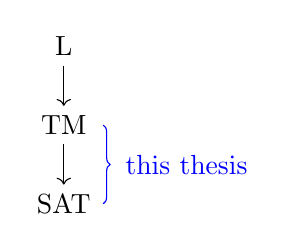
\begin{tikzpicture}
    \node (L) at (0, 3) {L};
    \node (TM) at (0, 2) {TM};
    \node (SAT) at (0, 1) {SAT};
    \draw[->] (L) -- (TM);
    \draw[->] (TM) -- (SAT);

    \draw[decorate, decoration={brace}, color=\colorTikzC] (0.5, 2) -- (0.5, 1) node[midway, xshift=1.0cm] {\colorHTwo{} this thesis};
  \end{tikzpicture}
\end{center}
\end{frame}

\begin{frame}{Generic Problem for Turing Machines}
  \begin{itemize}
    \item formalisation by~\cite{asperti_ricciotti} and mechanisation from~\cite{ForsterEtAl:2019:VerifiedTMs}
    \item two-sided infinite tapes
    \item no explicit blanks
  \end{itemize}

  \onslide<2->
  \begin{block}{\gennp{}}
    \vspace{-3ex}
    \begin{overlayarea}{\textwidth}{0.25\textwidth}
      \only<2>{
        \begin{align*}
          \gennp{}~&(M, \mathit{inp}, t) := M \text{ is a \emph{nondet.} 1-tape TM} \\
          \land & M \text{ accepts on } \mathit{inp} \text{ in } \le t \text{ steps}
        \end{align*}
      }
      \only<3->{
        \begin{align*}
          \gennp{}~&(M, \mathit{inp}, {\colorHTwo{}k'}, t) := M \text{ is a {\colorHTwo\emph{det.}} 1-tape TM} \\
          \land & {\colorHTwo{}\exists~\mathit{cert}, \length{cert} \le k'} \\
                & \land M \text{ accepts on } \mathit{inp}{\colorHTwo{}\concat\mathit{cert}} \text{ in } \le t \text{ steps}
        \end{align*}
      }
    \end{overlayarea}
  \end{block}
\end{frame}

\section{Tableau Construction}
\begin{frame}{Bounded Size}
  \sat{} formula has a fixed size, but: 
  \begin{itemize} 
    \item TM may have different space usage depending on input
    \item TM may take a different number of steps until it halts
  \end{itemize}
\end{frame}

\begin{frame}{Tableau of Configurations\footnote{based on\cite{Sipser:TheoryofComputation}, similar to \cite{Cook:1971:CTP:800157.805047}}}
  \begin{center}
    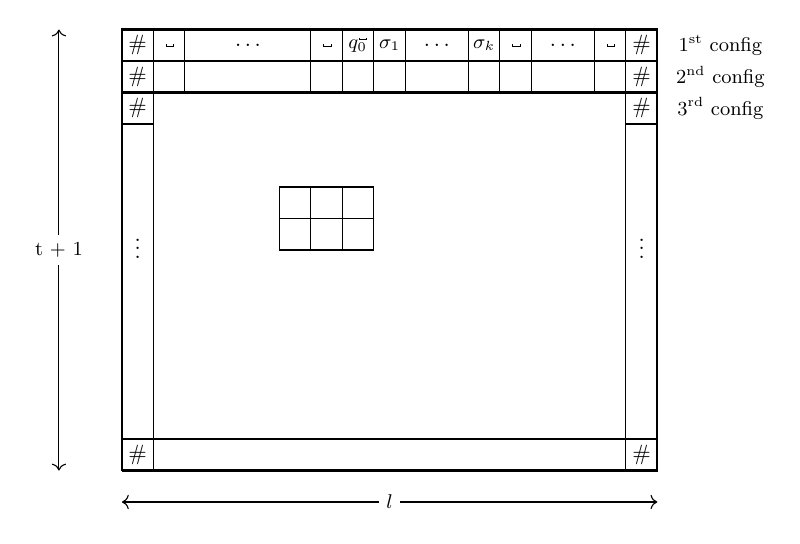
\begin{tikzpicture}[scale=0.8, every node/.style={scale=0.8}]
      \draw[thick] (1.5, -4) -- (1.5, 3) -- (10, 3) -- (10, -4) -- (1.5, -4);
      \draw (2, -4) -- (2, 3);
      \draw (2.5, 3) -- (2.5, 2);
      \draw (9.5, -4) -- (9.5, 3);
      \draw[thick] (1.5, 2.5) -- (10, 2.5);
      \draw[thick] (1.5, -3.5) -- (10, -3.5);
      \draw[thick] (1.5, 2) -- (10, 2);
      \draw[thick] (1.5, 1.5) -- (2, 1.5);
      \draw[thick] (9.5, 1.5) -- (10, 1.5);

      \draw (4.5, 3) -- (4.5, 2);
      \draw (5, 3) -- (5, 2);
      \draw (5.5, 3) -- (5.5, 2);
      \draw (6, 3) -- (6, 2);
      \draw (7, 3) -- (7, 2);
      \draw (7.5, 3) -- (7.5, 2);
      \draw (8, 3) -- (8, 2);
      \draw (9, 3) -- (9, 2);
      %\draw (2.5, 3) -- (2.5, 2);
      %\draw (3, 3) -- (3, 2.5);
      %\draw (4.5, 3) -- (4.5, 2.5);
      %\draw (5, 3) -- (5, 2.5);
      %\draw (5.5, 3) -- (5.5, 2.5);
      %\draw (7.5, 3) -- (7.5, 2.5);

      \node at (1.75, 2.75) {\#};
      \node at (1.75, 2.25) {\#};
      \node at (1.75, 1.75) {\#};
      \node at (1.75, -3.75) {\#};
      \node at (9.75, 2.75) {\#};
      \node at (9.75, 2.25) {\#};
      \node at (9.75, 1.75) {\#};
      \node at (9.75, -3.75) {\#};

      \node at (2.25, 2.75) {\textvisiblespace};
      \node at (3.5, 2.75) {$\ldots$};
      \node at (4.75, 2.75) {\textvisiblespace};
      \node at (5.25, 2.75) {\small $q_0^{\blank}$};
      \node at (5.75, 2.75) {\small $\sigma_1$};
      \node at (6.5, 2.75) {$\ldots$};
      \node at (7.25, 2.75) {\small $\sigma_k$};
      \node at (7.75, 2.75) {\textvisiblespace};
      \node at (8.5, 2.75) {$\ldots$};
      \node at (9.25, 2.75) {\textvisiblespace};

      %\node at (6.5, 2.75) {$\ldots$};
      %\node at (5, 2.25) {$\ldots$};

      \node at (1.75, -0.375) {$\vdots$};
      \node at (9.75, -0.375) {$\vdots$};

      \draw (4, -0.5) -- (4, 0.5) -- (5.5, 0.5) -- (5.5, -0.5) -- (4, -0.5);
      \draw (4.5, -0.5) -- (4.5, 0.5);
      \draw (5, -0.5) -- (5, 0.5);
      \draw (4, 0) -- (5.5, 0);

      \path[<->] (0.5, -4) edge node[fill=white, anchor=center, pos= 0.5] {\small t + 1} (0.5, 3);
      \path[<->] (1.5, -4.5) edge node[fill=white, anchor=center, pos=0.5] {\small $l$} (10, -4.5);
      %\path[<->] (5.5, 3.5) edge node[fill=white, anchor=center, pos=0.5] {\small $k$} (7.5, 3.5);

      \node at (11, 2.75) {\small 1\textsuperscript{st} config};
      \node at (11, 2.25) {\small 2\textsuperscript{nd} config};
      \node at (11, 1.75) {\small 3\textsuperscript{rd} config};
    \end{tikzpicture}
  \end{center} 
\end{frame}

\begin{frame}[t]{Configuration String}
  \begin{overlayarea}{\textwidth}{0.08\textwidth}
    %\color{gray}
    \begin{minipage}{0.48\textwidth}
      $\Sigma_{\text{TM}} = \{a, b, c\}$
    \end{minipage}
    \begin{minipage}{0.48\textwidth}
      \onslide<2->{
        \raggedleft
        $\delta(q_1, a) = (q_2, \Some{b}, \textsf{L})$
      }
    \end{minipage}
  \end{overlayarea}
  \begin{overlayarea}{\textwidth}{0.3\textwidth}
    \begin{center}
      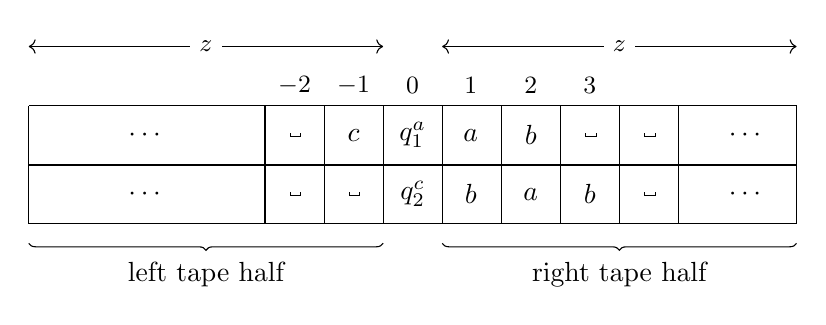
\begin{tikzpicture}
        \draw (0, 0.75) -- (9.75, 0.75);
        \draw (0, 0) -- (9.75, 0);
        \only<2->{
          \draw[thick] (0, 0) -- (9.75, 0);
        }
        \draw (0, 0) -- (0, 0.75);
        \draw (9.75, 0) -- (9.75, 0.75);

        \draw (4.5, 0) -- (4.5, 0.75);
        \draw (5.25, 0) -- (5.25, 0.75);
        \draw (3.75, 0) -- (3.75, 0.75);
        \draw (3, 0) -- (3, 0.75);
        \draw (6, 0) -- (6, 0.75);
        \draw (6.75, 0) -- (6.75, 0.75);
        \draw (7.5, 0) -- (7.5, 0.75);
        \draw (8.25, 0) -- (8.25, 0.75);

        \node at (5.6125, 1) {\small$1$};
        \node at (6.375, 1) {\small$2$};
        \node at (7.125, 1) {\small$3$};
        \node at (4.875, 1) {\small$0$};
        \node at (4.125, 1) {\small$-1$};
        \node at (3.375, 1) {\small$-2$};

        \node at (1.5, 0.375) {$\cdots$};
        \node at (9.125, 0.375) {$\cdots$};
        \node at (5.6125, 0.375) {$a$};
        \node at (6.375, 0.375) {$b$};
        \node at (7.125, 0.375) {\blank};
        \node at (7.875, 0.375) {\blank};
        \node at (4.875, 0.375) {$q_1^a$};
        \node at (4.125, 0.375) {$c$};
        \node at (3.375, 0.375) {\blank};

        \path[<->] (0, 1.5) edge node[fill=white, anchor=center, pos= 0.5] {\small $z$} (4.5, 1.5);
        \node[color=white] at (4.75, 1.5) {l};
        \path[<->] (5.25, 1.5) edge node[fill=white, anchor=center, pos =0.5] {\small $z$} (9.75, 1.5);

        \onslide<2-> {
          \draw (0, -0.75) -- (9.75, -0.75);
          \draw (0, -0.75) -- (0, 0);
          \draw (9.75, -0.75) -- (9.75, 0);

          \draw (4.5, 0) -- (4.5, -0.75);
          \draw (5.25, 0) -- (5.25, -0.75);
          \draw (3.75, 0) -- (3.75, -0.75);
          \draw (3, 0) -- (3, -0.75);
          \draw (6, 0) -- (6, -0.75);
          \draw (6.75, 0) -- (6.75, -0.75);
          \draw (7.5, 0) -- (7.5, -0.75);
          \draw (8.25, 0) -- (8.25, -0.75);

          \node at (1.5, -0.375) {$\cdots$};
          \node at (9.125, -0.375) {$\cdots$};
          \node at (5.6125, -0.375) {$b$};
          \node at (6.375, -0.375) {$a$};
          \node at (7.125, -0.375) {$b$};
          \node at (7.875, -0.375) {\blank};
          \node at (4.875, -0.375) {$q_2^c$};
          \node at (4.125, -0.375) {\blank};
          \node at (3.375, -0.375) {\blank};
        }

        \draw[decorate, decoration={brace, mirror}] (0, -1) -- (4.5, -1) node[midway, yshift=-0.4cm] {left tape half};
        \draw[decorate, decoration={brace, mirror}] (5.25, -1) -- (9.75, -1) node[midway, yshift=-0.4cm] {right tape half};
      \end{tikzpicture}
    \end{center}
  \end{overlayarea}
  \vspace{11ex}
  \emph{special blanks \blank{} for unused regions of the string}
\end{frame}

\begin{frame}[t]{Rewrite Windows: Force Valid Configuration Changes}
  \begin{overlayarea}{\textwidth}{0.08\textwidth}
    %\color{gray}
    \begin{minipage}{0.48\textwidth}
      $\Sigma_{\text{TM}} = \{a, b, c\}$
    \end{minipage}
    \begin{minipage}{0.48\textwidth}
      \onslide<1->{
        \raggedleft
        $\delta(q_1, a) = (q_2, \Some{b}, \textsf{L})$
      }
    \end{minipage}
  \end{overlayarea}
  \begin{overlayarea}{\textwidth}{0.3\textwidth}
    \begin{center}
      \begin{tikzpicture}
        \draw (0, 0.75) -- (9.75, 0.75);
        \draw[thick] (0, 0) -- (9.75, 0);
        \draw (0, 0) -- (0, 0.75);
        \draw (9.75, 0) -- (9.75, 0.75);

        \draw (4.5, 0) -- (4.5, 0.75);
        \draw (5.25, 0) -- (5.25, 0.75);
        \draw (3.75, 0) -- (3.75, 0.75);
        \draw (3, 0) -- (3, 0.75);
        \draw (6, 0) -- (6, 0.75);
        \draw (6.75, 0) -- (6.75, 0.75);
        \draw (7.5, 0) -- (7.5, 0.75);
        \draw (8.25, 0) -- (8.25, 0.75);

        \node at (5.6125, 1) {\small$1$};
        \node at (6.375, 1) {\small$2$};
        \node at (7.125, 1) {\small$3$};
        \node at (4.875, 1) {\small$0$};
        \node at (4.125, 1) {\small$-1$};
        \node at (3.375, 1) {\small$-2$};

        \node at (1.5, 0.375) {$\cdots$};
        \node at (9.125, 0.375) {$\cdots$};
        \node at (5.6125, 0.375) {\only<2-4>{\colorHTwo}$a$};
        \node at (6.375, 0.375) {\only<3-4>{\colorHTwo}$b$};
        \node at (7.125, 0.375) {\only<4>{\colorHTwo}\blank};
        \node at (7.875, 0.375) {\blank};
        \node at (4.875, 0.375) {\only<2-3>{\colorHTwo}$q_1^a$};
        \node at (4.125, 0.375) {\only<2>{\colorHTwo}$c$};
        \node at (3.375, 0.375) {\blank};

        \path[<->] (0, 1.5) edge node[fill=white, anchor=center, pos= 0.5] {\small $z$} (4.5, 1.5);
        \node[color=white] at (4.75, 1.5) {l};
        \path[<->] (5.25, 1.5) edge node[fill=white, anchor=center, pos =0.5] {\small $z$} (9.75, 1.5);

        \draw (0, -0.75) -- (9.75, -0.75);
        \draw (0, -0.75) -- (0, 0);
        \draw (9.75, -0.75) -- (9.75, 0);

        \draw (4.5, 0) -- (4.5, -0.75);
        \draw (5.25, 0) -- (5.25, -0.75);
        \draw (3.75, 0) -- (3.75, -0.75);
        \draw (3, 0) -- (3, -0.75);
        \draw (6, 0) -- (6, -0.75);
        \draw (6.75, 0) -- (6.75, -0.75);
        \draw (7.5, 0) -- (7.5, -0.75);
        \draw (8.25, 0) -- (8.25, -0.75);

        \node at (1.5, -0.375) {$\cdots$};
        \node at (9.125, -0.375) {$\cdots$};
        \node at (5.6125, -0.375) {\only<2-4>{\colorHTwo}$b$};
        \node at (6.375, -0.375) {\only<3-4>{\colorHTwo}$a$};
        \node at (7.125, -0.375) {\only<4>{\colorHTwo}$b$};
        \node at (7.875, -0.375) {\blank};
        \node at (4.875, -0.375) {\only<2-3>{\colorHTwo}$q_2^c$};
        \node at (4.125, -0.375) {\only<2>{\colorHTwo}\blank};
        \node at (3.375, -0.375) {\blank};

        \only<2>{
          \draw[color=\colorTikzC] (4.5, -0.75) -- (4.5, 0.75);
          \draw[color=\colorTikzC] (5.25, -0.75) -- (5.25, 0.75);
          \draw[color=\colorTikzC, thick] (3.75, 0) -- (6, 0);
        }
        \only<3>{
          \draw[color=\colorTikzC] (5.25, -0.75) -- (5.25, 0.75);
          \draw[color=\colorTikzC] (6, -0.75) -- (6, 0.75);
          \draw[color=\colorTikzC, thick] (4.5, 0) -- (6.75, 0);

        }
      \end{tikzpicture}
    \end{center}
  \end{overlayarea}

  \onslide<2->
  \begin{center}
    %\rewwin{\blank & \blank & c}{\blank & \blank & \blank}
    %\rewwin{\blank & c & q_1^a}{\blank & \blank & q_2^c}
    {
      \only<2>{\colorHTwo}
      \trewwin{c}{q_1^a}{a}{\blank}{q_2^c}{b}
    }
    \onslide<3->
    {
      \only<3>{\colorHTwo}
      \trewwin{q_1^a}{a}{b}{q_2^c}{b}{a}
    }
    \onslide<4->
    {
      \only<4>{\colorHTwo}
      \trewwin{a}{b}{\blank}{b}{a}{b}
    }
  \end{center}


\end{frame}

\begin{frame}{Parallel Rewriting (\PR{})}
  %\only<2->{\frametitle{Explicit Representation of Turing machines}}
  Given: 
  \begin{itemize}
    \item an initial string $x_0 \in \Sigma^l$ over an alphabet $\Sigma$ \\
      \onslide<1->{{\color{blue}{\emph{representation of initial config}}}}
    \item a set of rewrite windows $R$ of width $w$ \\ 
      \onslide<1->{{\color{blue}{\emph{possible local behaviours of the Turing machine}}}}
    \item a step count $t$ \\
      \onslide<1->{{\color{blue}\emph{number of TM steps}}}
    \item a set of final substring constraints $\Rfinal$ \\
      \onslide<1->{{\color{blue}\emph{symbols of accepting states}}}
  \end{itemize}
  Determine: $\exists$ $x_1, \ldots, x_t \in \Sigma^l$ s.t.\ 
  \begin{itemize}
    \item $x_i \rightsquigarrow x_{i+1}$: ``for all offsets there exists a rewrite window''
    \item there exists an element $x \in R_{\mathit{final}}$ which is a substring of $x_t$
  \end{itemize}
\end{frame}

\begin{frame}{Nondeterministic Certificate}
  \begin{itemize}
    \item ``guess'' certificate of length $\le k'$ with a single rewrite step
    \item add symbols $\{\underline{\#}, \underline{\blank}, \underline{*}, \underline{q^{\blank}}, \underline{\sigma}\}$ for initial state $q$ and $\sigma : \Sigma_{\textsf{TM}}$
  \end{itemize}

  \vspace{2ex}
  Initial string: 
  \begin{center}
  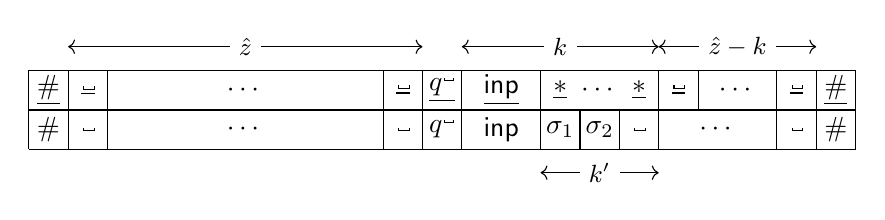
\begin{tikzpicture}[scale=1.0]
    \draw (0, 0.5) -- (10.5, 0.5);
    \draw[thick] (0, 0) -- (10.5, 0);
    \draw (0, 0) -- (0, 0.5);
    \draw (10.5, 0) -- (10.5, 0.5);

    \draw (0.5, 0.5) -- (0.5, 0);
    \draw (1, 0.5) -- (1, 0);
    \draw (10, 0.5) -- (10, 0);
    \draw (9.5, 0.5) -- (9.5, 0);
    \draw (5, 0.5) -- (5, 0);
    \draw (5.5, 0.5) -- (5.5, 0);
    \draw (4.5, 0.5) -- (4.5, 0);
    %\draw (6, 0.5) -- (6, 0);
    \draw (6.5, 0.5) -- (6.5, 0);
    %\draw (7, 0.5) -- (7, 0);
    %\draw (7.5, 0.5) -- (7.5, 0);
    \draw (8, 0.5) -- (8, 0);
    \draw (8.5, 0.5) -- (8.5, 0);

    \node at (9, 0.25) {$\cdots$};
    \node at (7.25, 0.25) {$\cdots$};
    \node at (2.75, 0.25) {$\cdots$};

    \node at (0.25, 0.25) {\underline{\#}};
    \node at (0.75, 0.24) {$\underline{\blank}$};
    \node at (4.75, 0.25) {$\underline{\blank}$};
    \node at (5.25, 0.25) {$\underline{q^{\blank}}$};
    \node at (6, 0.25) {\underline{\textsf{inp}}};
    \node at (6.75, 0.25) {$\underline{*}$};
    \node at (7.75, 0.25) {$\underline{*}$};
    \node at (8.25, 0.25) {$\underline{\blank}$};
    \node at (9.75, 0.25) {$\underline{\blank}$};
    \node at (10.25, 0.25) {\underline{\#}};

    \draw (0, -0.5) -- (10.5, -0.5);
    \draw (0, 0) -- (0, -0.5);
    \draw (10.5, 0) -- (10.5, -0.5);

    \draw (0.5, -0.5) -- (0.5, 0);
    \draw (1, -0.5) -- (1, 0);
    \draw (10, -0.5) -- (10, 0);
    \draw (9.5, -0.5) -- (9.5, 0);
    \draw (5, -0.5) -- (5, 0);
    \draw (5.5, -0.5) -- (5.5, 0);
    \draw (4.5, -0.5) -- (4.5, 0);
    %\draw (6, -0.5) -- (6, 0);
    \draw (6.5, -0.5) -- (6.5, 0);
    \draw (7, -0.5) -- (7, 0);
    \draw (7.5, -0.5) -- (7.5, 0);
    \draw (8, -0.5) -- (8, 0);
    %\draw (7.5, -0.5) -- (7.5, 0);
    %\draw (8, -0.5) -- (8, 0);
    %\draw (8.5, -0.5) -- (8.5, 0);

    \node at (2.75, -0.25) {$\cdots$};
    \node at (0.25, -0.25) {\#};
    \node at (0.75, -0.25) {\blank};
    \node at (4.75, -0.25) {\blank};
    \node at (5.25, -0.25) {$q^{\blank}$};
    \node at (6, -0.25) {\textsf{inp}};
    \node at (6.75, -0.25) {$\sigma_1$};
    \node at (7.25, -0.25) {$\sigma_2$};
    \node at (7.75, -0.25) {\blank};
    \node at (8.75, -0.25) {$\cdots$};
    \node at (9.75, -0.25) {\blank};
    \node at (10.25, -0.25) {\#};

    \path[<->] (5.5, 0.8) edge node[fill=white, anchor=center, pos= 0.5] {\small $k$} (8, 0.8);
    \path[<->] (0.5, 0.8) edge node [fill = white, anchor=center, pos=0.5] {\small $\hat{z}$} (5, 0.8);
    \path[<->] (8, 0.8) edge node [fill = white, anchor =center, pos=0.5] {\small $\hat{z}-k$} (10, 0.8);
    \path[<->] (6.5, -0.8) edge node[fill =white, anchor = center, pos = 0.5] {\small{$k'$}} (8, -0.8);
  \end{tikzpicture}
\end{center}
\end{frame}

\section{Encoding as CNF}

\begin{frame}<1-2>[label=chain]{Chain of Reductions}
  \begin{center}
    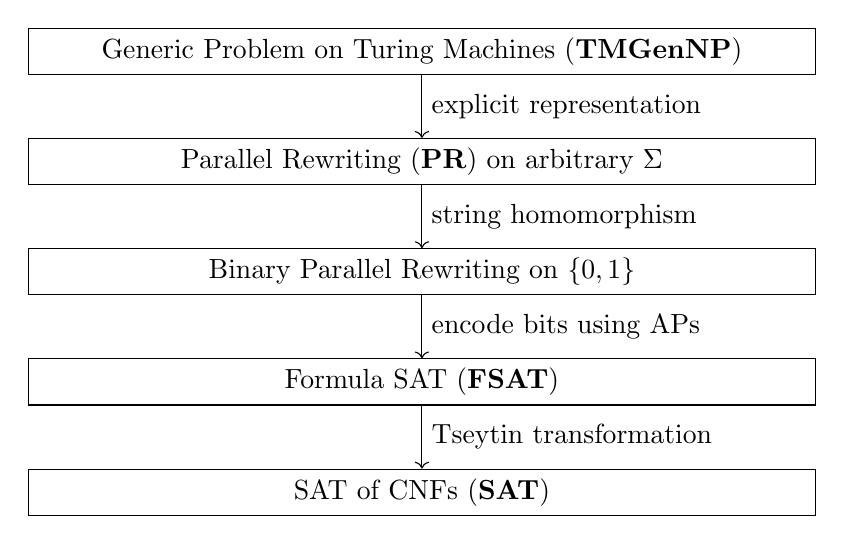
\begin{tikzpicture}[scale=1, every node/.style={scale=1}, node distance = 0.8cm]
      \node[rectangle, draw=black, minimum width=10cm] (gennp) {Generic Problem on Turing Machines (\gennp{})}; 
      \node[rectangle, draw=black, minimum width = 10cm, below = of gennp] (strrew1) {Parallel Rewriting (\PR{}) on arbitrary $\Sigma$};
      \draw[->] 
        (gennp) edge node[right] {explicit representation} (strrew1);

      \onslide<2->{ 
        \node[rectangle, draw=black, below = of strrew1, minimum width = 10cm] (strrew2) {Binary Parallel Rewriting on $\{0, 1\}$};
        \draw[->] 
          (strrew1) edge node[right] {string homomorphism} (strrew2);
      }
      \onslide<3->{
        \node[rectangle, draw=black, below = of strrew2, minimum width = 10cm] (csat) {Formula SAT (\fsat{})};
        \draw[->] 
         (strrew2) edge node[right] {encode bits using APs} (csat);

      }
      \onslide<4->{
        \node[rectangle, draw=black, below = of csat, minimum width = 10cm] (sat) {SAT of CNFs (\sat{})};
        \draw[->] 
          (csat) edge node[right] {Tseytin transformation} (sat);
      }
    \end{tikzpicture}
  \end{center}

\end{frame}

\begin{frame}{To a Binary Alphabet}
  \begin{itemize}
    \item arbitrary alphabet $\Sigma = \{\sigma_0, \ldots, \sigma_{\length{\Sigma} -1} \}$
    \item string homomorphism $h : \Sigma^* \rightarrow {\{0, 1\}}^*$ 
      \[\sigma_i \mapsto 0^i 1 0^{\length{\Sigma} - i - 1} \]
    \item in general: injective \emph{uniform} homomorphisms \\
      $\rightarrow$ scale length up by constant factor
  \end{itemize}

  Example ($\Sigma = \{a, b\}$):

  \begin{minipage}{0.48\textwidth}
    \begin{gather*}
      a \mapsto 01 \\
      b \mapsto 10
    \end{gather*}
  \end{minipage}
  \begin{minipage}{0.48\textwidth}
    \onslide<2->
    \begin{center}
      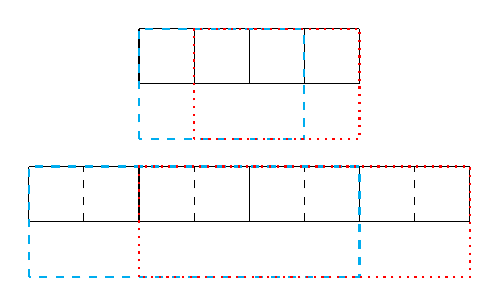
\begin{tikzpicture}[scale=0.7]
        \draw (0, 0) -- (4, 0);
        \draw (0, 1) -- (4, 1);
        \draw (0, 0) -- (0, 1); 
        \draw (4, 0) -- (4, 1);

        \draw (1, 0) -- (1, 1);
        \draw (2, 0) -- (2, 1);
        \draw (3, 0) -- (3, 1);

        \draw[dashed, thick, color=\colorTikzB] (0, -1) -- (0, 1) -- (3, 1) -- (3, -1) -- (0, -1);
        \draw[dotted, thick, color=\colorTikzA] (1,-1) -- (1, 1) -- (4, 1) -- (4, -1) -- (1, -1);

        \draw (-2, -2.5) -- (6, -2.5);
        \draw (-2, -1.5) -- (6, -1.5);
        \draw (-2, -2.5) -- (-2, -1.5); 
        \draw (6, -2.5) -- (6, -1.5);

        \draw[dashed] (1, -2.5) -- (1, -1.5);
        \draw (2, -2.5) -- (2, -1.5);
        \draw[dashed] (3, -2.5) -- (3, -1.5);
        \draw (4, -2.5) -- (4, -1.5);
        \draw[dashed] (5, -2.5) -- (5, -1.5);
        \draw (0, -2.5) -- (0, -1.5);
        \draw[dashed] (-1, -2.5) -- (-1, -1.5);

        \draw[dashed, thick, color=\colorTikzB] (-2, -3.5) -- (-2, -1.5) -- (4, -1.5) -- (4, -3.5) -- (-2, -3.5);
        \draw[dotted, thick, color=\colorTikzA] (0, -3.5) -- (0, -1.5) -- (6, -1.5) -- (6, -3.5) -- (0, -3.5);

      \end{tikzpicture}
    \end{center}
  \end{minipage}

\end{frame}

\againframe<3>{chain}

\newcommand{\bvar}{\textsf{var}}
\newcommand{\formula}{\mathcal{F}}
\newcommand{\encodesPred}{\textsf{encodesPredAt}}

\begin{frame}{Encoding as a Boolean Formula}
  \vspace{2ex}

  \begin{center}
    \begin{tikzpicture}
      \draw (1.5, -0.75) -- (1.5, 3) -- (10, 3) -- (10, -0.75) -- (1.5, -0.75);
      \draw (1.5, 2.25) -- (10, 2.25);
      \draw (1.5, 0) -- (10, 0);
      \draw (1.5, 1.5) -- (10, 1.5);

      \draw (2.5, 1.5) -- (2.5, 3);
      \draw (9, 1.5) -- (9, 3);
      \draw (2.5, 0) -- (2.5, -0.75);
      \draw (9, 0) -- (9, -0.75);
      
      \node at (2, 2.625) {\small$x_0$};
      \node at (9.5, 2.625) {\small$x_{l-1}$};
      \node at (2, 1.875) {\small$x_l$};
      \node at (9.5, 1.875) {\small$x_{2l-1}$};
      \node at (2, -0.375) {\small$x_{t\cdot l}$};
      %\node at (9.75, 0.25) {\small$x_{(t+1) \cdot m -1}$};

      \node at (5.75, -0.375) {$\cdots$};
      \node at (5.75, 2.625) {$\cdots$};
      \node at (5.75, 0.875) {$\vdots$};

      \path[<->] (0.75, -0.75) edge node[fill=white, anchor=center, pos= 0.5] {\small $t+1$} (0.75, 3);
      \path[<->] (1.5, -1.25) edge node[fill=white, anchor=center, pos=0.5] {\small $l$} (10, -1.25);
    \end{tikzpicture}     
  \end{center}

  $\Phi \defeq \Phi_{\textsf{init}} \land \Phi_{\textsf{rewrite}} \land \Phi_{\textsf{final}}$
  \begin{align*}
    \Phi_{\textsf{rewrite}} \defeq \bigwedge_{\text{rewrites}} \bigwedge_{\text{offsets}} \bigvee_{w \in R} \bigwedge_{\text{characters of } w} \textsf{encodeBit}
  \end{align*}

  \centering {\color{gray} $x_i \rightsquigarrow x_{i+1}$: ``for all offsets there exists a rewrite window''}
\end{frame}

\againframe<4>{chain}

\newcommand{\frepr}{\sdststile{}{}}
\section{Conclusion}

\begin{frame}{Contributions}
  \begin{block}{Main result}
    If \gennp{} is \NP{}-hard, then \SAT{} is \NP{}-complete. 
  \end{block}
  \begin{itemize}
    \item factorisation of the textbook proof~\cite{Sipser:TheoryofComputation} to make mechanisation feasible: new \PR{} problem
    \item full running-time analysis in L
  \end{itemize}

  Moreover: 
  \begin{itemize}
    \item $\gennp{} \in \NP{}$
    \item reduction $\text{$k$-\SAT{}} \redP{} \Clique{}$
    \item conditional \NP{}-completeness of $\Clique{}$
    \item formalisation of $\#P$
  \end{itemize}
\end{frame}

\begin{frame}{Future Work}
  \begin{itemize}
    \item missing reduction from L to \gennp{} 
    \item space-related results, e.g.\ Savitch
    %\item nondeterministic L
    %\item complexity theory beyond decision problems?
    \item binary encodings
  \end{itemize}
\end{frame}

\miniframesoff
\section{}

\newcommand{\BPR}{\textbf{BinaryPR}}
\begin{frame}{LOC}
  \vspace{-2ex}
  \begin{center}
  \begin{tabular}{cccc}
    \multicolumn{2}{c}{Component} & Spec & Proof \\
    \midrule
    \multicolumn{2}{c}{complexity definitions by Fabian} & 290 & 506 \\
    \midrule
    \multicolumn{2}{c}{preliminaries} & 281 & 634 \\
    \multicolumn{2}{c}{flat finite types} & 83 & 223 \\
    \multicolumn{2}{c}{problem definitions + \NP{} proofs} & 1093 & 1860\\ 
    \midrule
    \multirow{2}{*}{\gennp{} to \PR{}} & correctness & 1843 & 2481\\
     & time analysis & 838 & 1706 \\
    \multicolumn{2}{c}{\textbf{3-PR} to \PR{}} & 37 & 174 \\
    \multicolumn{2}{c}{\PR{} to \BPR{}} & 222 & 719 \\ 
    \multicolumn{2}{c}{\BPR{} to \fsat{}} & 312& 1078\\ 
    \multicolumn{2}{c}{\fsat{} to \SAT{}} & 213 & 605 \\ 
    \midrule
    \multicolumn{2}{c}{$k$-\SAT{} to \Clique{}} & 386 & 773 \\
    \midrule
      \multicolumn{2}{c}{total} & 5230 & 10038 \\
      \multicolumn{2}{c}{without extraction} & 3594 & 6857 \\
      \multicolumn{2}{c}{without computability} & 2339 & 4524

%for rt: 1636 / 3181 
%only correctness: 2339 / 4524

%preliminaries: preliminaries + polynomial bounds

  \end{tabular}
  \end{center}

\end{frame}

\begin{frame}[allowframebreaks]{Comparison with~\cite{gamboa:cook}}
  \begin{itemize}
    \item existing formalisation in ACL2 
    \item differences in setting: 
      \begin{itemize}
        \item single-sided infinite tapes 
        \item explicit nondeterminism instead of verifiers
        \item reduction only to \fsat{}
      \end{itemize}
    \item \emph{direct} reduction, no factorisation $\rightarrow$ only seems to be feasible because of restricted setting
    \item no running time analysis with respect to reasonable model
  \end{itemize}
\end{frame}

\begin{frame}[t]{Rewrite Rules}
  Add one symbol to the right half of the tape:
    \vspace{-0.5ex}
      \begin{center}
        \begin{tikzpicture}
          \draw (5.25, 0.75) -- (9.75, 0.75);
          \draw[thick] (5.25, 0) -- (9.75, 0);
          \draw (5.25, 0) -- (5.25, 0.75);
          \draw (9.75, 0) -- (9.75, 0.75);

          \draw (5.25, 0) -- (5.25, 0.75);
          \draw (6, 0) -- (6, 0.75);
          \draw (6.75, 0) -- (6.75, 0.75);
          \draw (7.5, 0) -- (7.5, 0.75);
          \draw (8.25, 0) -- (8.25, 0.75);

          \node at (9.125, 0.375) {$\cdots$};
          \node at (7.125, 0.375) {\blank};
          \node at (7.875, 0.375) {\blank};
          \only<1>{
            \node at (5.6125, 0.375) {$a$};
            \node at (6.375, 0.375) {$b$};
          }
          \only<2->{ 
            \node at (5.6125, 0.375) {$\sigma_1$};
            \node at (6.375, 0.375) {$\sigma_2$};
          }


          \draw (5.25, -0.75) -- (9.75, -0.75);
          \draw (5.25, -0.75) -- (5.25, 0);
          \draw (9.75, -0.75) -- (9.75, 0);

          \draw (5.25, 0) -- (5.25, -0.75);
          \draw (6, 0) -- (6, -0.75);
          \draw (6.75, 0) -- (6.75, -0.75);
          \draw (7.5, 0) -- (7.5, -0.75);
          \draw (8.25, 0) -- (8.25, -0.75);

          \node at (9.125, -0.375) {$\cdots$};
          \node at (7.875, -0.375) {$\blank$};
          \only<1>{
            \node at (5.6125, -0.375) {$b$};
            \node at (6.375, -0.375) {$a$};
            \node at (7.125, -0.375) {$b$};
          }
          \only<2->{
            \node at (5.6125, -0.375) {$\sigma_3$};
            \node at (6.375, -0.375) {$\sigma_1$};
            \node at (7.125, -0.375) {$\sigma_2$};
          }
        \end{tikzpicture}
        \end{center}
      \onslide<2->{
        \begin{center}
          $\sigma_i \in \Sigma_{\text{TM}}$
        \end{center}
      }

      \begin{center}
        \trewwin{\only<1>{a}\only<2->{\sigma_1}}{\only<1>{b}\only<2->{\sigma_2}}{\blank}{\only<1>{b}\only<2->{\sigma_3}}{\only<1>{a}\only<2->{\sigma_1}}{\only<1>{b}\only<2->{\sigma_2}}
        \onslide<3->{
          \trewwin{\sigma_2}{\blank}{\blank}{\sigma_1}{\sigma_2}{\blank}
          \trewwin{\blank}{\blank}{\blank}{\sigma_2}{\blank}{\blank}
          \vfill{}$\cdots$\vfill{}
        }
      \end{center}
\end{frame}



\begin{frame}[t]{Tape Shifts}
  Add one symbol to the right half of the tape:
  \begin{overlayarea}{\textwidth}{0.15\textwidth}
    \vspace{-0.5ex}
    \begin{minipage}{0.58\textwidth}
      \begin{center}
        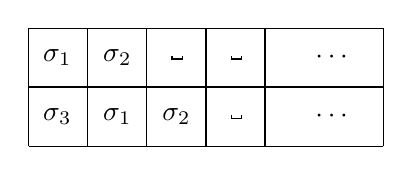
\begin{tikzpicture}
          \draw (5.25, 0.75) -- (9.75, 0.75);
          \draw[thick] (5.25, 0) -- (9.75, 0);
          \draw (5.25, 0) -- (5.25, 0.75);
          \draw (9.75, 0) -- (9.75, 0.75);

          \draw (5.25, 0) -- (5.25, 0.75);
          \draw (6, 0) -- (6, 0.75);
          \draw (6.75, 0) -- (6.75, 0.75);
          \draw (7.5, 0) -- (7.5, 0.75);
          \draw (8.25, 0) -- (8.25, 0.75);

          \node at (9.125, 0.375) {$\cdots$};
          \node at (7.125, 0.375) {\blank};
          \node at (7.875, 0.375) {\blank};

          \node at (5.6125, 0.375) {$\sigma_1$};
          \node at (6.375, 0.375) {$\sigma_2$};

          \draw (5.25, -0.75) -- (9.75, -0.75);
          \draw (5.25, -0.75) -- (5.25, 0);
          \draw (9.75, -0.75) -- (9.75, 0);

          \draw (5.25, 0) -- (5.25, -0.75);
          \draw (6, 0) -- (6, -0.75);
          \draw (6.75, 0) -- (6.75, -0.75);
          \draw (7.5, 0) -- (7.5, -0.75);
          \draw (8.25, 0) -- (8.25, -0.75);

          \node at (9.125, -0.375) {$\cdots$};
          \node at (7.875, -0.375) {\blank};
          \node at (5.6125, -0.375) {$\sigma_3$};
          \node at (6.375, -0.375) {$\sigma_1$};
          \node at (7.125, -0.375) {$\sigma_2$};
        \end{tikzpicture}
        \only<2->{
          \begin{tikzpicture}[overlay, remember picture]
            \node at (4.5, 0.8) {$\sigma_i \in \Sigma_{\text{TM}}$ };
          \end{tikzpicture}
        }
      \end{center}
    \end{minipage}
    \begin{minipage}{0.38\textwidth}
      \trewwin{\sigma_1}{\sigma_2}{\blank}{\sigma_3}{\sigma_1}{\sigma_2}
    \end{minipage}
  \end{overlayarea}

  \vspace{2ex}

  \onslide<3->
  Leave the tape unchanged:

  \begin{overlayarea}{\textwidth}{0.15\textwidth}
    \vspace{-0.5ex}
    \begin{minipage}{0.58\textwidth}
      \begin{center}
        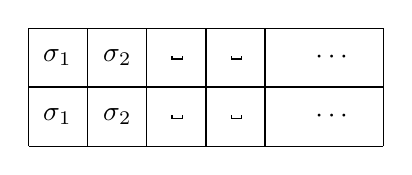
\begin{tikzpicture}
          \draw (5.25, 0.75) -- (9.75, 0.75);
          \draw[thick] (5.25, 0) -- (9.75, 0);
          \draw (5.25, 0) -- (5.25, 0.75);
          \draw (9.75, 0) -- (9.75, 0.75);

          \draw (5.25, 0) -- (5.25, 0.75);
          \draw (6, 0) -- (6, 0.75);
          \draw (6.75, 0) -- (6.75, 0.75);
          \draw (7.5, 0) -- (7.5, 0.75);
          \draw (8.25, 0) -- (8.25, 0.75);

          \node at (9.125, 0.375) {$\cdots$};
          \node at (7.125, 0.375) {\blank};
          \node at (7.875, 0.375) {\blank};
          \node at (5.6125, 0.375) {$\sigma_1$};
          \node at (6.375, 0.375) {$\sigma_2$};


          \draw (5.25, -0.75) -- (9.75, -0.75);
          \draw (5.25, -0.75) -- (5.25, 0);
          \draw (9.75, -0.75) -- (9.75, 0);

          \draw (5.25, 0) -- (5.25, -0.75);
          \draw (6, 0) -- (6, -0.75);
          \draw (6.75, 0) -- (6.75, -0.75);
          \draw (7.5, 0) -- (7.5, -0.75);
          \draw (8.25, 0) -- (8.25, -0.75);

          \node at (9.125, -0.375) {$\cdots$};
          \node at (7.125, -0.375) {\blank};
          \node at (7.875, -0.375) {\blank};
          \node at (5.6125, -0.375) {$\sigma_1$};
          \node at (6.375, -0.375) {$\sigma_2$};
        \end{tikzpicture}
      \end{center}
    \end{minipage}
    \begin{minipage}{0.38\textwidth}
      \only<5>{\colorHOne}
      \trewwin{\sigma_1}{\sigma_2}{\blank}{\sigma_1}{\sigma_2}{\blank}
    \end{minipage}
  \end{overlayarea}

  \vspace{2ex}
  \onslide<4->
  \begin{center}

    \begin{tikzpicture}
      \draw (0, 0.75) -- (9.75, 0.75);
      \draw[thick] (0, 0) -- (9.75, 0);
      \draw (0, 0) -- (0, 0.75);
      \draw (9.75, 0) -- (9.75, 0.75);

      \draw (4.5, 0) -- (4.5, 0.75);
      \draw (5.25, 0) -- (5.25, 0.75);
      \draw (3.75, 0) -- (3.75, 0.75);
      \draw (3, 0) -- (3, 0.75);
      \draw (6, 0) -- (6, 0.75);
      \draw (6.75, 0) -- (6.75, 0.75);
      \draw (7.5, 0) -- (7.5, 0.75);
      \draw (8.25, 0) -- (8.25, 0.75);

      %\node at (5.6125, 1) {\small$1$};
      %\node at (6.375, 1) {\small$2$};
      %\node at (7.125, 1) {\small$3$};
      %\node at (4.875, 1) {\small$0$};
      %\node at (4.125, 1) {\small$-1$};
      %\node at (3.375, 1) {\small$-2$};

      \node at (1.5, 0.375) {$\cdots$};
      \node at (9.125, 0.375) {$\cdots$};
      \node at (5.6125, 0.375) {\only<5>{\colorHOne}\only<6->{\colorHTwo}$b$};
      \node at (6.375, 0.375) {\only<5>{\colorHOne}\only<6->{\colorHTwo}$b$};
      \node at (7.125, 0.375) {\only<5>{\colorHOne}\blank};
      \node at (7.875, 0.375) {\blank};
      \node at (4.875, 0.375) {\only<6->{\colorHTwo}$q_1^a$};
      \node at (4.125, 0.375) {$c$};
      \node at (3.375, 0.375) {\blank};

      %\path[<->] (0, 1.5) edge node[fill=white, anchor=center, pos= 0.5] {\small $z$} (4.5, 1.5);
      %\node[color=white] at (4.75, 1.5) {l};
      %\path[<->] (5.25, 1.5) edge node[fill=white, anchor=center, pos =0.5] {\small $z$} (9.75, 1.5);

      \draw (0, -0.75) -- (9.75, -0.75);
      \draw (0, -0.75) -- (0, 0);
      \draw (9.75, -0.75) -- (9.75, 0);

      \draw (4.5, 0) -- (4.5, -0.75);
      \draw (5.25, 0) -- (5.25, -0.75);
      \draw (3.75, 0) -- (3.75, -0.75);
      \draw (3, 0) -- (3, -0.75);
      \draw (6, 0) -- (6, -0.75);
      \draw (6.75, 0) -- (6.75, -0.75);
      \draw (7.5, 0) -- (7.5, -0.75);
      \draw (8.25, 0) -- (8.25, -0.75);

      \only<6->{ 
        \draw[color=\colorTikzC, thick] (4.5, 0) -- (6.75, 0);
        \draw[color=\colorTikzC] (5.25, -0.75) -- (5.25, 0.75);
        \draw[color=\colorTikzC] (6, -0.75) -- (6, 0.75);
      }
      \only<5> {
        \draw[color=\colorTikzA, thick] (5.25, 0) -- (7.5, 0);
        \draw[color=\colorTikzA] (6, -0.75) -- (6, 0.75);
        \draw[color=\colorTikzA] (6.75, -0.75) -- (6.75, 0.75);
      }

      \node at (1.5, -0.375) {$\cdots$};
      \node at (9.125, -0.375) {$\cdots$};
      \node at (5.6125, -0.375) {\only<5>{\colorHOne{}}\only<6->{\colorHTwo}$b$};
      \node at (6.375, -0.375) {\only<4>{b}\only<5->{\only<5>{\colorHOne{}}\only<6->{\colorHTwo}$b$}};
      \node at (7.125, -0.375) {\only<4>{b}\only<5->{\only<5>{\colorHOne{}}\blank}};
      \node at (7.875, -0.375) {\blank};
      \node at (4.875, -0.375) {\only<6->{\colorHTwo}$q_2^c$};
      \node at (4.125, -0.375) {\blank};
      \node at (3.375, -0.375) {\blank};
    \end{tikzpicture}
  \end{center}
\end{frame}

\begin{frame}{Polarities $\{\overset{\leftarrow}{\cdot}, \overset{-}{\cdot}, \overset{\rightarrow}{\cdot}\}$}
  Add one symbol to the right half of the tape:
  \begin{overlayarea}{\textwidth}{0.15\textwidth}
    \vspace{-0.5ex}
    \begin{minipage}{0.58\textwidth}
      \begin{center}
        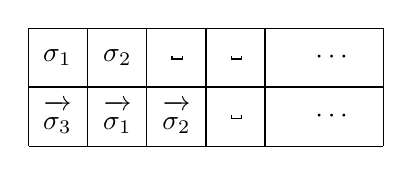
\begin{tikzpicture}
          \draw (5.25, 0.75) -- (9.75, 0.75);
          \draw[thick] (5.25, 0) -- (9.75, 0);
          \draw (5.25, 0) -- (5.25, 0.75);
          \draw (9.75, 0) -- (9.75, 0.75);

          \draw (5.25, 0) -- (5.25, 0.75);
          \draw (6, 0) -- (6, 0.75);
          \draw (6.75, 0) -- (6.75, 0.75);
          \draw (7.5, 0) -- (7.5, 0.75);
          \draw (8.25, 0) -- (8.25, 0.75);

          \node at (9.125, 0.375) {$\cdots$};
          \node at (7.125, 0.375) {\blank};
          \node at (7.875, 0.375) {\blank};

          \node at (5.6125, 0.375) {$\sigma_1$};
          \node at (6.375, 0.375) {$\sigma_2$};


          \draw (5.25, -0.75) -- (9.75, -0.75);
          \draw (5.25, -0.75) -- (5.25, 0);
          \draw (9.75, -0.75) -- (9.75, 0);

          \draw (5.25, 0) -- (5.25, -0.75);
          \draw (6, 0) -- (6, -0.75);
          \draw (6.75, 0) -- (6.75, -0.75);
          \draw (7.5, 0) -- (7.5, -0.75);
          \draw (8.25, 0) -- (8.25, -0.75);

          \node at (9.125, -0.375) {$\cdots$};
          \node at (7.875, -0.375) {\blank};
          \node at (5.6125, -0.375) {$\polpos{\sigma_3}$};
          \node at (6.375, -0.375) {$\polpos{\sigma_1}$};
          \node at (7.125, -0.375) {$\polpos{\sigma_2}$};
        \end{tikzpicture}
      \end{center}
    \end{minipage}
    \begin{minipage}{0.38\textwidth}
      \trewwin{\sigma_1}{\sigma_2}{\blank}{\polpos{\sigma_3}}{\polpos{\sigma_1}}{\polpos{\sigma_2}}
    \end{minipage}
  \end{overlayarea}

  \vspace{2ex}

  Leave the tape unchanged:

  \begin{overlayarea}{\textwidth}{0.15\textwidth}
    \vspace{-0.5ex}
    \begin{minipage}{0.58\textwidth}
      \begin{center}
        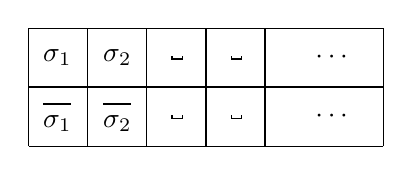
\begin{tikzpicture}
          \draw (5.25, 0.75) -- (9.75, 0.75);
          \draw[thick] (5.25, 0) -- (9.75, 0);
          \draw (5.25, 0) -- (5.25, 0.75);
          \draw (9.75, 0) -- (9.75, 0.75);

          \draw (5.25, 0) -- (5.25, 0.75);
          \draw (6, 0) -- (6, 0.75);
          \draw (6.75, 0) -- (6.75, 0.75);
          \draw (7.5, 0) -- (7.5, 0.75);
          \draw (8.25, 0) -- (8.25, 0.75);

          \node at (9.125, 0.375) {$\cdots$};
          \node at (7.125, 0.375) {\blank};
          \node at (7.875, 0.375) {\blank};
          \node at (5.6125, 0.375) {$\sigma_1$};
          \node at (6.375, 0.375) {$\sigma_2$};


          \draw (5.25, -0.75) -- (9.75, -0.75);
          \draw (5.25, -0.75) -- (5.25, 0);
          \draw (9.75, -0.75) -- (9.75, 0);

          \draw (5.25, 0) -- (5.25, -0.75);
          \draw (6, 0) -- (6, -0.75);
          \draw (6.75, 0) -- (6.75, -0.75);
          \draw (7.5, 0) -- (7.5, -0.75);
          \draw (8.25, 0) -- (8.25, -0.75);

          \node at (9.125, -0.375) {$\cdots$};
          \node at (7.125, -0.375) {\blank};
          \node at (7.875, -0.375) {\blank};
          \node at (5.6125, -0.375) {$\polneut{\sigma_1}$};
          \node at (6.375, -0.375) {$\polneut{\sigma_2}$};
        \end{tikzpicture}
      \end{center}
    \end{minipage}
    \begin{minipage}{0.38\textwidth}
      \trewwin{\sigma_1}{\sigma_2}{\blank}{\polneut{\sigma_1}}{\polneut{\sigma_2}}{\blank}
    \end{minipage}
  \end{overlayarea}

  \vspace{2ex}
  \onslide<2->
  \begin{center}

    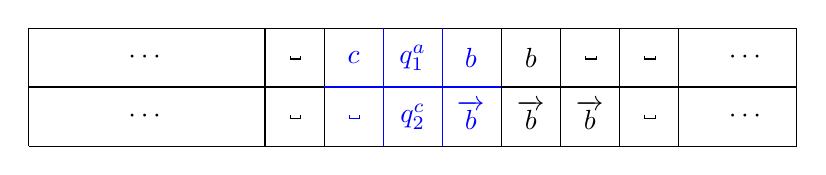
\begin{tikzpicture}
      \draw (0, 0.75) -- (9.75, 0.75);
      \draw[thick] (0, 0) -- (9.75, 0);
      \draw (0, 0) -- (0, 0.75);
      \draw (9.75, 0) -- (9.75, 0.75);

      \draw (4.5, 0) -- (4.5, 0.75);
      \draw (5.25, 0) -- (5.25, 0.75);
      \draw (3.75, 0) -- (3.75, 0.75);
      \draw (3, 0) -- (3, 0.75);
      \draw (6, 0) -- (6, 0.75);
      \draw (6.75, 0) -- (6.75, 0.75);
      \draw (7.5, 0) -- (7.5, 0.75);
      \draw (8.25, 0) -- (8.25, 0.75);

      %\node at (5.6125, 1) {\small$1$};
      %\node at (6.375, 1) {\small$2$};
      %\node at (7.125, 1) {\small$3$};
      %\node at (4.875, 1) {\small$0$};
      %\node at (4.125, 1) {\small$-1$};
      %\node at (3.375, 1) {\small$-2$};

      \node at (1.5, 0.375) {$\cdots$};
      \node at (9.125, 0.375) {$\cdots$};
      \node[color=\colorTikzC] at (5.6125, 0.375) {$b$};
      \node at (6.375, 0.375) {$b$};
      \node at (7.125, 0.375) {\blank};
      \node at (7.875, 0.375) {\blank};
      \node[color=\colorTikzC] at (4.875, 0.375) {$q_1^a$};
      \node[color=\colorTikzC] at (4.125, 0.375) {$c$};
      \node at (3.375, 0.375) {\blank};

      %\path[<->] (0, 1.5) edge node[fill=white, anchor=center, pos= 0.5] {\small $z$} (4.5, 1.5);
      %\node[color=white] at (4.75, 1.5) {l};
      %\path[<->] (5.25, 1.5) edge node[fill=white, anchor=center, pos =0.5] {\small $z$} (9.75, 1.5);
      \draw (0, -0.75) -- (9.75, -0.75);
      \draw (0, -0.75) -- (0, 0);
      \draw (9.75, -0.75) -- (9.75, 0);

      \draw (4.5, 0) -- (4.5, -0.75);
      \draw (5.25, 0) -- (5.25, -0.75);
      \draw (3.75, 0) -- (3.75, -0.75);
      \draw (3, 0) -- (3, -0.75);
      \draw (6, 0) -- (6, -0.75);
      \draw (6.75, 0) -- (6.75, -0.75);
      \draw (7.5, 0) -- (7.5, -0.75);
      \draw (8.25, 0) -- (8.25, -0.75);

      \draw[color=\colorTikzC, thick] (3.75, 0) -- (6, 0);
      \draw[color=\colorTikzC] (4.5, -0.75) -- (4.5, 0.75);
      \draw[color=\colorTikzC] (5.25, -0.75) -- (5.25, 0.75);

      \node at (1.5, -0.375) {$\cdots$};
      \node at (9.125, -0.375) {$\cdots$};
      \node[color=\colorTikzC] at (5.6125, -0.375) {$\polpos{b}$};
      \node at (6.375, -0.375) {$\polpos{b}$};
      \node at (7.125, -0.375) {$\polpos{b}$};
      \node at (7.875, -0.375) {\blank};
      \node[color=\colorTikzC] at (4.875, -0.375) {$q_2^c$};
      \node[color=\colorTikzC] at (4.125, -0.375) {\blank};
      \node at (3.375, -0.375) {\blank};
    \end{tikzpicture}
  \end{center}
\end{frame}

\begin{frame}{Transition Rules -- Example}
  \onslide<2>{In Coq mechanisation:}
  \begin{tikzpicture}[overlay, remember picture]
    \node at (5, 1.17) {$m \in \Sigma_{\text{TM}} \cup \{\blank\}, \sigma \in \Sigma_{\text{TM}}$};
  \end{tikzpicture}

  $\delta(q, a) = (p, \Some{b}, L)$: 
  \begin{overlayarea}{\textwidth}{0.7\textheight}
    \only<1>{
      \begin{center}
        \trewwin{\blank}{q^{a}}{m_1}{\blank}{p^{\blank}}{\polpos{b}}
        \trewwin{\sigma_1}{q^a}{m_1}{\polpos{m_2}}{p^{\sigma_1}}{\polpos{b}}\\
        \trewwin{\blank}{\blank}{q^a}{\blank}{\blank}{p^{\blank}}
        \trewwin{\blank}{\sigma_1}{q^a}{\blank}{\blank}{p^{\sigma_1}}
        \trewwin{\sigma_1}{\sigma_2}{q^a}{\polpos{m_1}}{\polpos{\sigma_1}}{p^{\sigma_2}} \\
        \trewwin{q^a}{\blank}{\blank}{p^{m_1}}{\polpos{b}}{\blank}
        \trewwin{q^a}{\sigma_1}{m_1}{p^{m_2}}{\polpos{b}}{\polpos{\sigma_1}}
      \end{center}
    }
    \only<2->{
      \begin{center}
        \trewwin{m_1}{q^a}{m_2}{\polpos{m_3}}{p^{m_1}}{\polpos{b}}
        \trewwin{m_1}{m_2}{q^a}{\polpos{m_3}}{\polpos{m_1}}{p^{m_2}}
        \trewwin{q^a}{m_1}{m_2}{p^{m_3}}{\polpos{b}}{\polpos{m_1}}
      \end{center}

      Induces garbage, e.g. 
      \begin{center}
        \trewwin{\blank}{q^a}{\blank}{\polpos{\sigma}}{p^{\blank}}{\polpos{b}}
      \end{center}
    }
  \end{overlayarea}
\end{frame}

\begin{frame}{Representation Relations}
  Representation of tape halves: 
  \begin{center}
    $u \sim_t^{n} $
    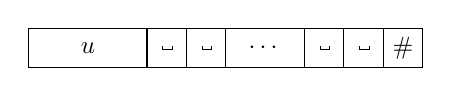
\begin{tikzpicture}[scale=0.5, every node/.style={scale=0.9}, baseline=(base), inner sep = 0pt]
      \node (base) at (0, 0.3) {};
      \draw (0, 0) -- (0, 1) -- (10, 1) -- (10, 0) -- (0, 0);
      \draw (3, 0) -- (3, 1);
      \draw (4, 0) -- (4, 1);
      \draw (5, 0) -- (5, 1);
      \draw (7, 0) -- (7, 1);
      \draw (8, 0) -- (8, 1);
      \draw (9, 0) -- (9, 1);

      \node at (1.5, 0.5) {$u$};
      \node at (3.5, 0.5) {\blank};
      \node at (4.5, 0.5) {\blank};
      \node at (6, 0.5) {$\cdots$};
      \node at (7.5, 0.5) {\blank};
      \node at (8.5, 0.5) {\blank};
      \node at (9.5, 0.5) {\#};

    \end{tikzpicture}\\
    \begin{tikzpicture}[remember picture, overlay]
      \draw[decorate, decoration={brace, mirror}, xshift=-2cm, yshift=0.7cm] (0, -0.5) -- (3.5, -0.5) node[midway, yshift=-0.4cm] {$n$};
    \end{tikzpicture}
  \end{center}

  \vspace{3ex}

  Representation of configurations:

  \begin{center}
  $q; (ls, \sigma, rs) \sim_c $
  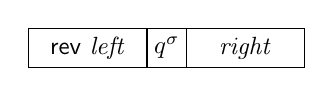
\begin{tikzpicture}[scale=0.5, every node/.style={scale=0.9}, baseline=(base), inner sep = 0pt]
    \node (base) at (0, 0.3) {};
    \draw (0, 0) -- (7, 0);
    \draw (0, 1) -- (7, 1);
    \draw (0, 0) -- (0, 1);
    \draw (7, 0) -- (7, 1);

    \draw (3, 0) -- (3, 1);
    \draw (4, 0) -- (4, 1);

    \node at (1.5, 0.5) { $\rev~\mathit{left}$ };
    \node at (5.5, 0.5) { $\mathit{right}$ };
    \node at (3.5, 0.5) { $q^\sigma$ };
  \end{tikzpicture}, where: 
\end{center}
  \begin{itemize}
    \item $ls \sim_t^{z'} \mathit{left}$
    \item $rs \sim_t^{z'} \mathit{right}$
  \end{itemize}

\end{frame}

\begin{frame}{Deterministic Simulation}
  \begin{center}
    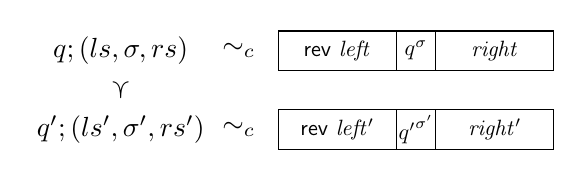
\begin{tikzpicture}
      \node at (0, 0.5) {$q; (ls, \sigma, rs)$};
      \node at (0, -0.5) {$q'; (ls', \sigma', rs')$};
      \node[rotate=270] at (0, 0) {$\succ$};

      \draw[scale=0.5] (4, 0.5) -- (11, 0.5);
      \draw[scale=0.5] (4, 1.5) -- (11, 1.5);
      \draw[scale=0.5] (4, 0.5) -- (4, 1.5);
      \draw[scale=0.5] (11, 0.5) -- (11, 1.5);

      \draw[scale=0.5] (7, 0.5) -- (7, 1.5);
      \draw[scale=0.5] (8, 0.5) -- (8, 1.5);

      \node[scale=0.8] at (2.75, 0.5) { $\rev~\mathit{left}$ };
      \node[scale=0.8] at (4.75, 0.5) { $\mathit{right}$ };
      \node[scale=0.8] at (3.75, 0.5) { $q^\sigma$ };

      \node[rotate=270] at (3.75, 0) {$\rightsquigarrow$};

      \draw[scale=0.5] (4, -0.5) -- (11, -0.5);
      \draw[scale=0.5] (4, -1.5) -- (11, -1.5);
      \draw[scale=0.5] (4, -0.5) -- (4, -1.5);
      \draw[scale=0.5] (11, -0.5) -- (11, -1.5);

      \draw[scale=0.5] (7, -0.5) -- (7, -1.5);
      \draw[scale=0.5] (8, -0.5) -- (8, -1.5);

      \node[scale=0.8] at (2.75, -0.5) { $\rev~\mathit{left'}$ };
      \node[scale=0.8] at (4.75, -0.5) { $\mathit{right'}$ };
      \node[scale=0.8] at (3.75, -0.5) { ${q'}^{\sigma'}$ };

      \node at (1.5, 0.5) {$\sim_c$};
      \node at (1.5, -0.5) {$\sim_c$};
    \end{tikzpicture}
  \end{center}
  where $ls \sim_t^{z'} \mathit{left}, rs \sim_t^{z'} \mathit{right}$ and $ls' \sim_t^{z'} \mathit{left'}, rs' \sim_t^{z'} \mathit{right'}$


  \onslide<2->{
    \begin{center}
      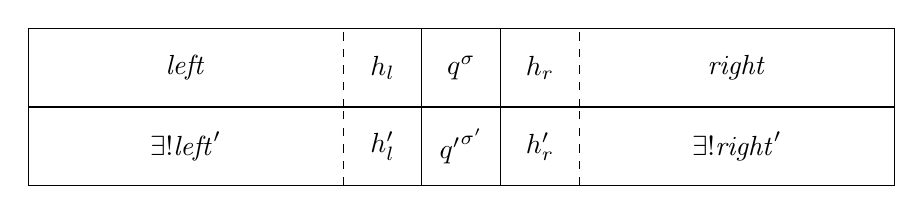
\begin{tikzpicture}
        \draw (0, 0) -- (11, 0);
        \draw (0, 1) -- (11, 1);
        \draw (0, 0) -- (0, 1);
        \draw (11, 0) -- (11, 1);

        \draw (5, 0) -- (5, 1);
        \draw (6, 0) -- (6, 1);

        \onslide<3->{
          \draw[dashed] (7, 0) -- (7, 1);
          \draw[dashed] (4, 0) -- (4, 1);
          \node at (4.5, 0.5) {$h_l$};
          \node at (6.5, 0.5) {$h_r$};
        }

        \node at (2, 0.5) {$\mathit{left}$};
        \node at (9, 0.5) {$\mathit{right}$};
        \node at (5.5, 0.5) {$q^\sigma$};

        \onslide<4-> {
          \draw (4, -1) -- (7, -1);
          \draw (5, -1) -- (5, 0);
          \draw (6, -1) -- (6, 0);

          \draw[dashed] (7, -1) -- (7, 0);
          \draw[dashed] (4, -1) -- (4, 0);

          \node at (4.5, -0.5) {$h_l'$};
          \node at (6.5, -0.5) {$h_r'$};
          \node at (5.5, -0.5) {${q'}^{\sigma'}$};
        }

        \onslide<5-> {
          \draw (0, -1) -- (0, 0);
          \draw (11, -1) -- (11, 0);
          \draw (0, -1) -- (4, -1);
          \draw (7, -1) -- (11, -1);

          \node at (2, -0.5) {$\exists! \mathit{left}'$};
          \node at (9, -0.5) {$\exists! \mathit{right}'$};
        }

    \end{tikzpicture}
  \end{center}
}
%Somehow portray the idea that everything (flow of information) is propagated from the center of the string; the rewrite is determined uniquely by the head.

%Then: rewrites for tape halves can be proven separately using only a subset of the rules

\end{frame}


\begin{frame}{Tape Transformations}
  Add symbol: 
  \[ rs \reprt{} h \land |rs| < z' \rightarrow \exists! h', (h \rightsquigarrow \polpos{a} :: h') \land a :: rs \reprt{+} \polpos{a} :: h' \]
  \[ ls \reprt{} h \land |ls| < z' \rightarrow \exists! h', (\rev{h} \rightsquigarrow \rev{\polneg{a} :: h'}) \land a :: ls \reprt{-} \polneg{a} :: h'
  \]
  
  Remove symbol: 
  \[a :: b :: rs \reprt{} a :: b :: h \rightarrow \exists! h', (a :: b :: h \rightsquigarrow \polneg{b} :: h') \land b :: rs \reprt{-} \polneg{b} :: h' \]

  Leave unchanged:
  \[a :: rs \reprt{} a :: h \rightarrow \exists! h', (a :: h \rightsquigarrow \polneut{a} :: h) \land a :: rs \reprt{\circ} \polneut{a} :: h' \]

\end{frame}

\begin{frame}{Main Simulation Results}
  \begin{block}{Completeness}
    Let $(q, \mathit{tape})$ be a configuration with $\length{tape} \le k$. There exists $s$ with $(q, \mathit{tape}) \reprc{} s$.

    If $(q, \mathit{tape}) \triangleright^{\le t} (q', \mathit{tape}')$, then there exists $s'$ with $s \rightsquigarrow^t s'$, $(q', \mathit{tape}') \reprc{} s'$ and $s' \models \Rfinal$. 
  \end{block}

  \begin{block}{Soundness}
    Let $s$ be given such that $(q, \mathit{tape}) \reprc{} s$ and $\length{\mathit{tape}} \le k$ for some $q, \mathit{tape}$. 

    If $s \rightsquigarrow^t s'$ and $s' \models \Rfinal$, then there exists $(q', \mathit{tape}')$ with $(q', \mathit{tape}') \reprc{} s'$ such that $(q, \mathit{tape}) \triangleright^{\le t} (q', \mathit{tape}')$ and $\length{\mathit{tape}'} \le z'$. 
  \end{block}
\end{frame}

\begin{frame}{Formulas: Representation of Predicates}
  \vspace{-3ex}
  \[f : \formula \defeq \btrue \bnfmid v \bnfmid f_1 \lor f_2 \bnfmid f_1 \land f_2 \bnfmid \lnot f \qquad (v : \bvar{} \defeq \nat) \]
  \vspace{3ex}

  \begin{itemize}
    \item explicit assignments $e : \listsof{\bool}$ to variables $[s, s + \length{e})$
    \item encoding of predicates $p : \listsof{\bool} \rightarrow \Prop$: \[\encodesPred~\textsf{start}~l~f~p \defeq \forall a, a \models f \leftrightarrow p~(a[\textsf{start}, \textsf{start} + l])\]
    \item $\textsf{encodeBit}~\textsf{var}~\textsf{bit} \defeq \ITE{\textsf{bit}}{\textsf{var}}{\lnot \textsf{var}}$
      \[\encodesPred~v~1~(\textsf{encodeBit}~v~b) (\lambda e. e = [s]) \]
  \end{itemize} 
\end{frame}



\newcommand{\Frepr}[3]{\sdststile{\ensuremath{#3}}{\ensuremath{#1, #2}}}
\begin{frame}[t]{The Tseytin Transformation}
  Goal: convert formula to CNF \\
  Example: $f = f_1 \lor f_2$
  \vspace{2ex}

  \begin{overlayarea}{\textwidth}{0.4\textwidth}
    \only<1-4>{
      Naive approach: 
      \begin{align*}
        f = f_1 \lor f_2 \leadsto &\alt<1>{\phantom{(C_1}N_1\phantom{C_2)} \lor \phantom{(C_3}N_2\phantom{C_4)}}{(C_1 \land C_2)\lor (C_3 \land C_4)} \\
        \onslide<3->{ \leftrightarrow & (C_1 \lor C_3) \land (C_1 \lor C_4) \land (C_2 \lor C_3) \land (C_2 \land C_4) }
      \end{align*}
      \onslide<4>{{\colorHOne exponential blowup!}}
    }

    \only<5->{ 
      \emph{Solution:} introduce new variables: $f \mapsto (v, N)$ s.t. 
      \[f \frepr{} (v, N) \defeq \SAT{} f \leftrightarrow \SAT (v \land N) \]
      \vspace{-2ex}
      \onslide<6->{
        \begin{gather*}
          f_1 \frepr{} (v_1, N_1) \qquad f_2 \frepr{} (v_2, N_2) \\
          \text{Goal: } f = f_1 \lor f_2 \frepr{} (v, N) \text{ for fresh } v \\
          \only<7-> { 
            N \defeq \underbrace{N_1}_{f_1 \leftrightarrow v_1} \land \underbrace{N_2}_{f_2 \leftrightarrow v_2} \land \alt<-7>{?\phantom{(\leftrightarrow (v_1 \lor v_2))}}{(v \leftrightarrow (v_1 \lor v_2))} \\ 
            \only<8->{\Rightarrow f \leftrightarrow v}
          }
        \end{gather*}
      }
    }
  \end{overlayarea}

  \vspace{5ex}
  \[\scalebox{0.9}{$N : \textsf{cnf} \qquad C : \textsf{clause} \qquad v : \textsf{var} \qquad f: \formula{}$} \]
\end{frame}


\begin{frame}{Tseytin: Correctness Relation}
  \[ \textsf{tseytin}' : \underbrace{\textsf{var}}_{\text{next free var}} \rightarrow \formula{} \rightarrow \underbrace{\textsf{var}}_{\text{representing variable}} \times \textsf{cnf} \times \underbrace{\textsf{var}}_{\text{next free var}} \] 
  
  \[ f \Frepr{nf}{nf'}{b} (v, N), \text{ iff } \]
  \begin{itemize} 
    \item $N \subseteq ([0, b) \cup [nf, nf'))$,
    \item $v \in [nf, nf')$,
    \item for all $a \subseteq [0, b)$, there exists $a' \subseteq [nf, nf')$ such that $(a \cup a') \models N$,
    \item and for all $a$ with $a \models N$, the equivalence $a \models v \leftrightarrow a \models f$ holds.
  \end{itemize}
\end{frame}

\begin{frame}{Basic Definitions: \NP{}\footnote{Definitions by Fabian}}
  Problem $Q : X \rightarrow \Prop$

  \vspace{2ex}
  $Q \in \NP{}$ iff:
  \begin{itemize}
    \item there is a verifier $V : X \rightarrow Y \rightarrow \Prop$
    \item $V$ is polynomial-time computable 
      %(in $\textsf{size}(\overline x), \textsf{size}(\overline{cert})$)
    \item $V$ verifies $Q$ 
      \begin{itemize}
        \item $V~x~y \rightarrow Q~x$
        \item $Q~x \rightarrow \exists y, V~x~y$ and $y$ has polynomial size 
    %\item $\exists (p : \nat \rightarrow \nat), \forall x~\mathit{cert}, V~x~\mathit{cert} \rightarrow \textsf{size}(\overline {\mathit{cert}}) \le p(\textsf{size}(\overline x))$
    %\item $V$ only accepts certificates of polynomial size
      \end{itemize}
  \end{itemize}
\end{frame}

\begin{frame}{Basic Definitions: Polynomial-Time Reductions\footnote{Definitions by Fabian}}
  \[P : X \rightarrow \Prop \qquad Q : Y \rightarrow \Prop\]

  \begin{align*}
    P \redP{} Q := \exists f : X \rightarrow Y, \quad&(\forall x, P~x \leftrightarrow Q(f~x)) \\
    \land& \text{ polynomial-time computable } f\\
    \onslide<2->{\land &~f \text{ increases the size polynomially}} 
  \end{align*}
  
  \onslide<3->{
    \begin{align*}
      \textsf{NP-hard}~P \defeq \forall Q, Q \in \NP{} \rightarrow Q \redP{} P \\
      \textsf{NP-complete}~P \defeq P \in \NP{} \land \textsf{NP-hard}~P 
    \end{align*}
  }
\end{frame}

\newcommand*{\eval}{\mathcal{E}}
\newcommand*{\evalA}[2]{\eval~#1~#2}
\newcommand{\encsize}[1]{\left\lVert#1\right\rVert}
\newcommand{\nil}{[~]}

\begin{frame}{Proving Time Bounds}
  \begin{align*}
    \textsf{cnf} &\defeq \listsof{\textsf{clause}} \\
    \eval_N &: \textsf{assgn} \rightarrow \textsf{cnf} \rightarrow \bool \\
    \eval_N~a~\nil{} &\defeq \btrue{} \\
    \eval_N~a~(C::N) &\defeq \eval_C~a~C~\&~\eval_N~a~N 
  \end{align*}

  \begin{enumerate}[1.]
    \item extraction, running time in terms of arguments
      \begin{align*}
        T(\eval_N)~a~\nil &\ge 9 \\
        T(\eval_N)~a~(C :: N) &\ge T(\eval_N)~a~N + T (\eval_C)~a~C + 22
      \end{align*}
    \item bound by monotonic polynomial $p_{\eval_N} : \nat \rightarrow \nat$ s.t.\
      \[\forall a~N, T_{\eval_N}~a~N \le p_{\eval_N}(\encsize{\overline{a}} + \encsize{\overline{N}}) \]
      in this case: 
      $p_{\eval_N}(n) \defeq n \cdot p_{\eval_C}(n) + c_{\eval_N} \cdot (n +1)$
  \end{enumerate}
\end{frame}

\newcommand{\SharpP}{\textsf{\#P}}
\begin{frame}{\SharpP}
  counting problem $f : X \rightarrow \nat$

  \begin{block}{Verifier Characterisation of \SharpP}
    $f \in \SharpP$, iff there exists a verifier $R : X \rightarrow Y \rightarrow \Prop$ s.t.\ 
    \begin{itemize}
      \item $R$ runs in polynomial time
      \item $R$ only accepts certificates of a polynomial size
      \item $\forall x, \length{\{y~|~R~x~y\}} = f~x$
    \end{itemize}
  \end{block}

  finite cardinalities $\length{\{y~|~R~x~y\}}$ defined using listability\\[2ex]

  Shortcomings: 
  \begin{itemize}
    \item only computable counting problems definable (solution: functional relations)
    \item precise definition of counting problems requires a bit of care (e.g. \textbf{\#SAT})
  \end{itemize}
\end{frame}

%\begin{frame}{possible other stuff}
  %\begin{itemize}
    %\item 2-PR vs 3-PR
    %\item explain fixed state symbol
    %\item size explosion as reason for using TM
  %\end{itemize}
%\end{frame}

\begin{frame}[allowframebreaks]{References}
  \nocite{Sipser:TheoryofComputation}
  \nocite{Bläser:TISkript}
  \bibliographystyle{apalike}
  \bibliography{references}{}
\end{frame}
\end{document}
